\documentclass[12pt,a4paper]{article}

\usepackage[utf8]{inputenc}
\usepackage[portuguese]{babel}
\usepackage[T1]{fontenc}
\usepackage[left=2.5cm,right=2.5cm,top=2cm,bottom=2cm]{geometry}
%\usepackage{fancyhdr}
%\pagestyle{fancy}
\usepackage{graphicx}
\usepackage{color}
\usepackage{indentfirst}
\usepackage{wrapfig}
\usepackage{lipsum}
\usepackage{setspace}
\usepackage{adjustbox}
\usepackage{minted}
\usepackage{amsmath}
\bibliographystyle{unsrtnat}
\usepackage[numbers,sort&compress]{natbib}
\usepackage{breakcites}
\usepackage[breaklinks=true]{hyperref}
\usepackage{hyperref}

\usepackage{microtype} % Improves typography
\usepackage{gfsdidot} % Use the GFS Didot font: http://www.tug.dk/FontCatalogue/gfsdidot/


% Create a new command for the horizontal rule in the document which allows thickness specification
\makeatletter
\def\vhrulefill#1{\leavevmode\leaders\hrule\@height#1\hfill \kern\z@}
\makeatother
\parindent 1cm

 \renewcommand{\rmdefault}{phv} % Arial
 \renewcommand{\sfdefault}{phv} % Arial

\title{Relatório PIBIC Daniel Benvenutti}
%\author{}

\thispagestyle{empty}

\begin{document}


\begin{wrapfigure}[2]{l}{10cm}
\begin{center}
    
\includegraphics[scale=1]{banner-grande.png}
\end{center}

\end{wrapfigure}






\noindent 
\begin{flushright}
\begin{scriptsize}
\hspace{5cm} \\
\hspace{5cm} \\
\hspace{5cm} \\
\hspace{5cm} \\
\hspace{5cm} \\
\hspace{5cm} \\
% Instituto de Física Gleb Watghin\\
% Rua Sergio Buarque de Holanda, 777\\
% 13083-859, Campinas, SP \\
% e-mail: rouxinol@unicamp.br\\
% tel: +55(19)3521-5462\\
% \hspace{-0.5cm} 
% \vhrulefill{1pt} \\ % 
\end{scriptsize}
\end{flushright}

% \singlespacing %Para um espaçamento simples
% \onehalfspacing %Para um espaçamento de 1,5
%\doublespacing %Para um espaçamento duplo 

% $ $\\


% \singlespacing %Para um espaçamento simples
% \large 
\begin{flushleft}
\textbf{Projeto Principal}: “Algoritmo quântico de busca de Grover e de fatoração de Shor: implementação da simulação em computadores clássicos e quânticos”\\
\textbf{Grande Área de conhecimento:} Ciências Exatas e da Terra\\
% \textbf{Grande Área de conhecimento: }Ciências Exatas e da Terra\\
\textbf{Área de Conhecimento:} Física\\
\textbf{Subárea de Conhecimento: }Física da Matéria Condensada\\
\textbf{Aluno(a):} Daniel Benvenutti (169448) - \url{danielgb23@gmail.com}\\
\textbf{Orientador: }Francisco Rouxinol - \url{rouxinol@ifi.unicamp.br}\\
\textbf{Instituição:} Instituto de Física Gleb Wataghin, UNICAMP\\
\textbf{Palavras chaves:} Eletrodinâmica Quântica, Computação Quântica e Informação\\
\textbf{Referente:} Relatório XXVIII Congresso de Iniciação Científica da UNICAMP
\end{flushleft}


%  \singlespacing %Para um espaçamento simples
\abstract{\textbf{Resumo do projeto original:} Nós apresentamos um projeto de pesquisa focado no desenvolvimento pelo aluno de um conjunto de ferramentas para simular algoritmos quânticos em computadores clássicos e quânticos. Serão tratados e discutidos os conceitos básicos de computação quântica e mecânica quântica, como também a implementação de portas quânticas e o algoritmo de busca de Groover e de Shor. Com a implementação deste projeto é esperado que importantes conceitos de quântica, como medida, funções de onda de muitos corpos, e momento angular, sejam aprofundados como também o estudo de importantes tópicos avançados em física e engenharia. }

\singlespacing %Para um espaçamento simples
\section*{Resumo Ilustrado}
\begin{figure}[h!]
    \centering
    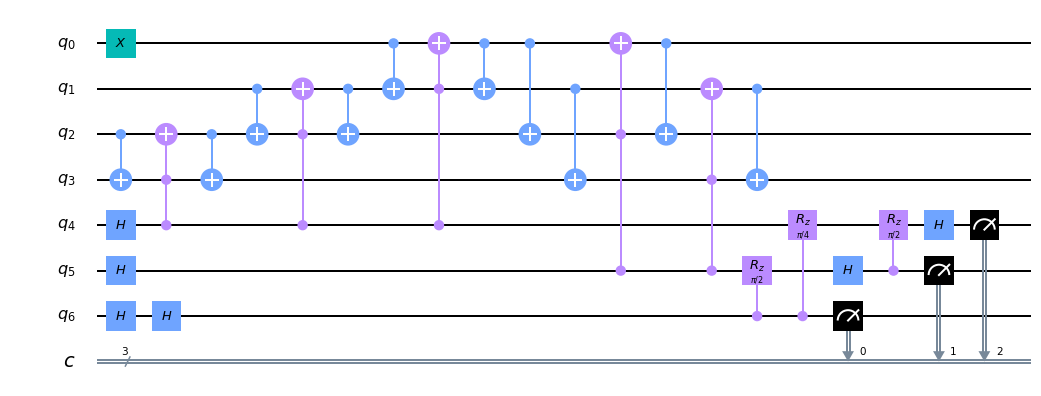
\includegraphics[width=0.9\textwidth]{shora2draw.png}
 
    \label{fig:groovercq}
\end{figure}
Computação quântica combina ciência da computação com mecânica quântica, possibilitando a realização de certos cálculos exponencialmente mais rápido do que as contrapartes clássicas, fazendo uso da superposição quântica e emaranhamento de estados quânticos
Neste circuito apresentamos o Algoritmo de Shor para fatorar C=15 com a=2 que foi executado no computador quântico da IBM \textit{ibmq 16 melbourne}. Neles temos 3 Hadamards de superposição nos qubits do expoente, um circuito de CNOTs e Toffollis para multiplicar a base e o circuito de transformada de Fourier quântica inversa nos qubits do expoente também



\newpage

\section{Atividades Principais}

 Inicialmente desenvolvemos os registradores de N-qubits. Cada registrador guardava a informação do estado composto por 3 sistemas de dois níveis (qubits), descrito por um único estado quântico conjunto $|\psi\rangle$.  Utilizando estes vetores, preparamos algorítimos para preparar o sistema de interesse no estado de interesse. 

Na segunda etapa, desenvolvemos funções que simulam uma porta quântica (análogo a uma porta lógica), necessárias para operar os qubits. Utilizando os elementos dos vetores de estado e a portas lógicas, a probabilidade de medir um determinado valor pode ser determinado, simulando-se uma medida no sistema quântico. 

Com estas funções e algorítimos programados, foram preparados os algorítimos de Grover de busca e Shor de fatoração de números inteiros. Ambos funcionaram como esperado. 

Na última implementamos os algorítimos Groover de busca e Shor de fatoração de números inteiros no computador quântico da IBM e comparamos com os resultados obtidos em nosso programa.

Fornecemos o código utilizando nesta etapa na plataforma GitHub no endereço: \url{https://github.com/Danielgb23/ic_comp_quantica}
% {https://github.com/Danielgb23/ic_comp_quantica/blob/master/caderno_qiskit_comp_real.ipynb}

\subsection{Registrador Quântico}
A primeira parte do projeto e construir o simulador. Para simular o estado de $N$ qubits precisamos de um vetor de  $2^{N}$ elementos. Cada estado nesse vetor representa uma combinação das medidas possíveis dos qubits e superposições das mesmas. A probabilidade de cada medida é representada pelo quadrado do módulo(complexo) de cada elemento do vetor.

\subsection{Portas quânticas}
Uma das portas quânticas mais importantes é a \textit{Porta de Hadamard}, $H$. Ela é extremamente interessante, pois coloca um qubit em uma superposição de dois estados. 

Outra importante porta é a \textit{Porta de Fase}, $S$.  Ela muda a fase complexa do elemento $|1\rangle$ do vetor que descreve o qubit.


 Portões CNOT são portas quânticas NOT (ou NÃO) controladas e funcionam da seguinte maneira: Há um qubit controlador e um qubit que sofre a operação NOT. Se e somente se o qubit controlador é $|1\rangle$ que o outro qubit é invertido . Se o controlador for $|0\rangle$ o controlado mantém o seu estado. O qubit controlador não é alterado. Com essa porta podemos fazer o estado de emaranhamento quântico.
 



\subsection{Algoritmo de Groover}
O algoritmo de Groover é um algoritmo de busca. Dado um vetor de possíveis respostas,  procuramos neste vetor, um valor específico, que indica qual é a resposta correta. 
Com uma algoritmo normal de varredura em um computador clássico no pior caso temos que verificar todos os $n$ elementos. Já no algoritmo de Groover precisamos de apenas $\sqrt{n}$ buscas.
O algoritmo de Groover funciona usando uma técnica chamada amplificação de amplitude. Que tem esse nome pois o algoritmo amplifica a amplitude da resposta no vetor de estados.

O construção dele é baseado em dois estágios. Primeiro colocamos todos os qubits em superposição (todas as medidas com mesma probabilidade). Depois vem o oráculo e o bloco de difusão de Grover. Que temos que repetir juntos $\frac{\pi}{4} 2^{N_{qubits}}$ vezes (arredondado). O oráculo inverte a amplitude quântica da resposta e o bloco de difusão amplifica o que estiver invertido.

Em seguida avaliamos o desempenho da simulação do algoritmo de Groover no meu computador. Abaixo os resultados:

\begin{table}[htb]

\begin{adjustbox}{center}
\begin{tabular}{|l|l|}  
\hline
Qubits  & tempo \\ \hline
1  & 1.20s \\ \hline
2  &  1.15s\\ \hline
3  &   1.36s\\ \hline
4  &  3.51s\\ \hline
5  &  29.33s\\ \hline
6  &   353.69s\\ \hline

\end{tabular}
\end{adjustbox}
\caption{Tempos de simulação de Grover para diferentes números de qubits}
\end{table}


Depois o algoritmo de Groover foi executado utilizando-se matrizes esparsas. Que são muito úteis nessas simulações, já que as matrizes dos operadores têm muitos zeros.


\begin{table}[htb]
\centering
\begin{adjustbox}{center}
\begin{tabular}{|l|l|}  
\hline
Qubits  & tempo \\ \hline
1  & 0.86s \\ \hline
2  &  0.92s\\ \hline
3  &   0.91s\\ \hline
4  &  0.97s\\ \hline
5  &  1.04s\\ \hline
6  &   1.16s\\ \hline

\end{tabular}
\end{adjustbox}
\caption{Tempos de simulação de Grover para diferentes números de qubits utilizando matrizes esparsas}
\end{table}

Nota-se a grande melhoria no desempenho e como é possível utilizar um número muito maior de qubits com o mesmo computador.

\subsection{Algoritmo de Shor}
 O algoritmo de Shor é um algoritmo de fatoração de números inteiros. Um dos seus passos é acelerado se executado em um computador quântico.  O resto dos passos são feitos rapidamente em um computador clássico. A algoritimo se fundamenta no fato de que dado um $C$ que se deseja encontrar os fatores e um $a$ escolhido segundo algumas regras se encontrarmos um período $p$ da função $a^p \, mod \, C$ par e não satisfaça $a^{p/2} \equiv -1\, mod\, C$. $P_{\pm} = mdc( a^{p/2} \pm 1, C)$ são fatores não triviais de C. A parte quântica encontra $p$. 
 
 Para essa parte quântica dividimos os qubits em expoente e base. Depois executamos três divisões do circuito: a primeira faz a superposição de todos os qubits do expoente(para entrar como todos os valores possíveis ao mesmo tempo).
 
 Depois multiplicamos a base que está inicializada em $|1\rangle$ sucessivamente par cada qubit do expoente por $a^{2^W V_{qubit}} $ onde $2^W$ e o peso binário do qubit (exemplo $101_b=2^2+1=5_d$ então o peso do primeiro qubit é 4) e $V_{qubit}$ é zero ou um dependendo do valor desse qubit.
 
 Finalmente aplicamos a transformada quântica de Fourier inversa(IQFT). O que obtemos das operações anteriores é uma função semelhante a um pente em uma superposição dos vários valores para a base e com um período $\omega$. A IQFT muda-a para o domínio da frequência e obtemos a frequência equivalente ao inverso do período $f=1/\omega$ e suas harmônicas (2f, 3f, ...) como resultado(ver figura \ref{fig:Shor1} com período 4 e frequência de 1/4).  \cite{Candela2015UndergraduateComputing}
 
\begin{figure}
    \centering
    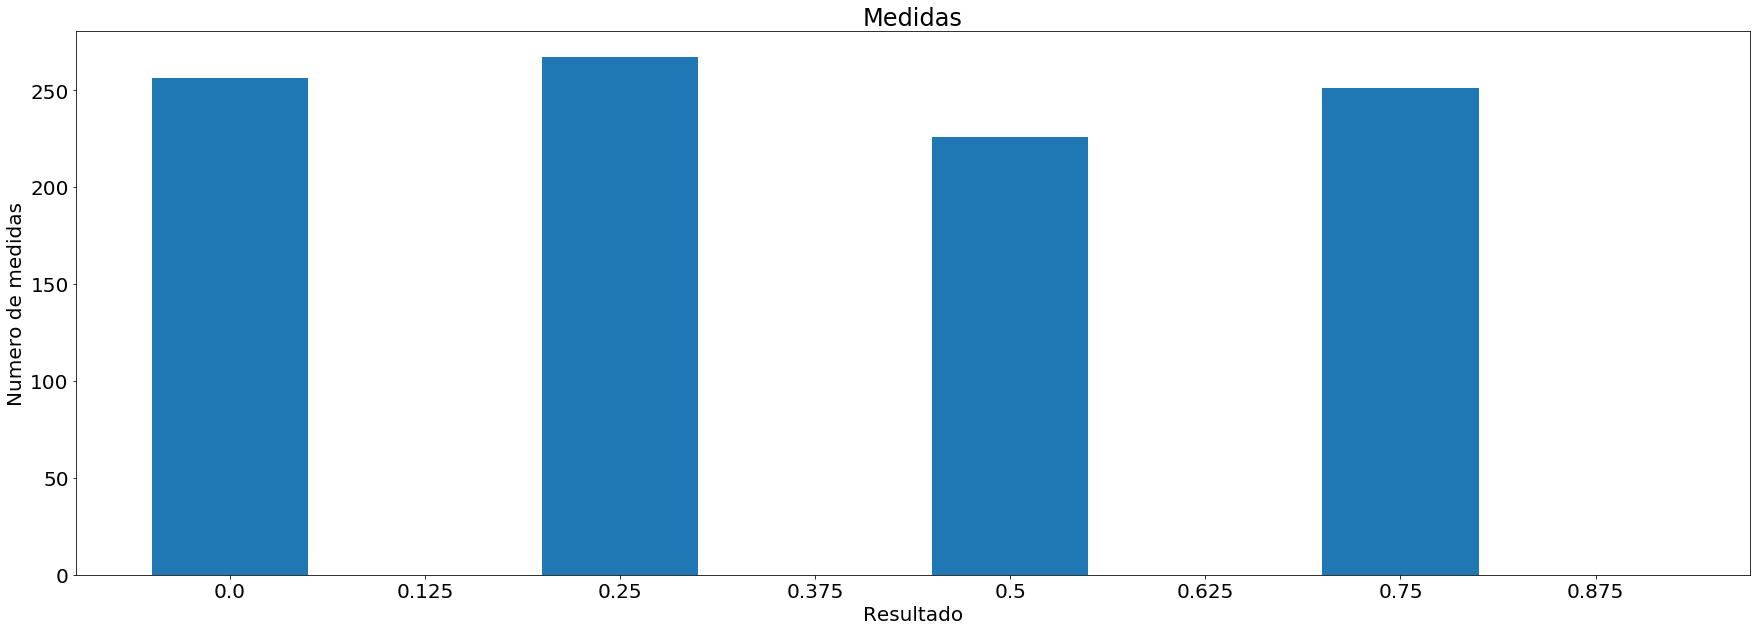
\includegraphics[width=1\textwidth]{relatorio-shor1.png}
    \caption{Histograma com valores obtidos para a aplicação do algoritmo de Shor com 7 qubits fatorando 15 com a=2}
    \label{fig:Shor1}
\end{figure}

 


\subsection{Implementação no computador Quântico}
Após a simulação do qubits foram utilizados os computadores quânticos disponibilizados pela IBM na IBM Quantum experience \cite{IBM2019IBMExperience}. Foram demonstrados os Algoritmos de Groover e Shor executados nessas máquinas. Tiveram de ser utilizadas novas portas quânticas enquanto outras não estão disponíveis na mesma forma da simulação no computador apresentando desafios. Outro desafio é a limitação física das máquinas da IBM.  A linguagem utilizada para programar essas máquinas foi o Qiskit que é baseada em python. 

\subsubsection{Algoritmo de Groover}
Para executar o algoritmo de Groover na máquina da IBM temos duas limitações principais. A primeira é que o algoritmo fica longo a medida que aumentamos o número de qubits. Isso porque precisamos repetir uma parte do circuito $\pi/4\sqrt{2^N}$ vezes arredondado onde N é o número de qubits. O que já deixa o circuito longo para a máquina da IBM se usarmos 3 qubits.  E dependendo da máquina que utilizarmos como a IBM Q 14 Melbourne que tem mais qubits,  portanto é mais suscetível a ruídos, já será muito mais difícil de distinguir a solução. 

A segunda limitação são as portas que podemos utilizar. Numa simulação com matrizes fica simples fazer uma porta que inverte a fase de apenas um elemento da base mas agora temos que implementar isso com outras portas quânticas fundamentais. Felizmente para três qubits podemos usar uma porta Z controlada por dois qubits que pode ser feita com uma porta de Toffoli e duas de Hardamard nas entradas do qubit que será negado. Essa porta inverte a fase do componente $|111\rangle$ apenas. Para usar em outros componentes podemos colocar portas NOT na entrada e saída dessa porta para que mude a fase de outra combinação de qubits. 

\subsubsection{Algoritmo de Shor}
No algoritmo de Shor a maior limitação para a implementação em um computador quântico real é a porta quântica que faz a multiplicação por $a^x\,mod\,C$. Já que temos que implementá-la através de outras portas mais fundamentais e não diretamente através da matriz como na simulação. 

Primeiro implementei um circuito mais simples com 5 qubits usando $C=15$ e $a=4$ que têm um período de apenas 2 o que permite encolher bastante o circuito.

Para fazer o multiplicador por $a^x\, mod\, 15=4^x\, mod\, 15$. Dividimos ele em duas partes: $4^1\, mod\, 15$ controlado pelo qubit de $x$ menos significativo e $4^2\, mod\, 15$ controlado pelo mais significativo. Assim se o qubit de $x$ menos significativo for 1 multiplicamos $f$ por $4\,mod\,15$ e o mesmo para o mais. Obtendo assim $4^{x_0+x_1}\, mod\, 15$. Como $4^2\,mod\,15=16\,mod\,15=1$ precisamos fazer apenas o do bit menos significativo. Para multiplicar o número 1 por 4 sempre que o qubit menos significativo de $x$ for 1 basta usar uma porta CNOT que zera a porta com 1 do digito menos significativo com peso 1 e uma que seta o qubit com peso 4.

Agora executamos o algoritmo com a=2 o que vai requerer 6 qubits.
O novo multiplicador é assim: $a^x\, mod\, 15=2^x\, mod\, 15$. Dividimos ele em 3 partes: $2^1\, mod\, 15$ controlado pelo qubit de $x$ menos significativo, $2^2\, mod\, 15$ controlado pelo qubit do meio e $2^4\, mod\, 15$ controlado pelo mais significativo. Assim se o qubit de $x$ menos significativo for 1 multiplicamos $f$ por $2\,mod\,15$ e o mesmo para os outros. Obtendo assim $4^{x_0+x_1+x_2}\, mod\, 15$. Como $2^4\,mod\,15=16\,mod\,15=1$ precisamos fazer apenas o do meio e o do qubit menos significativo. Para multiplicar um número por 2 módulo 15 vamos usar três portas de Fredkin. 
Para números binários, a multiplicação por dois é um deslocamento para a esquerda. Como fazemos o módulo 15 do valor também note que os números dão a volta pela esquerda de volta a direta, como uma rotação. Para fazer esse deslocamento usamos portas de Fredkin para fazer SWAPs controlados nos qubits de $f$. Para multiplicar por $2^2=4$ o circuito vai funcionar de maneira semelhante. Só que com um deslocamento de dois qubits.

\section{Conclusões}
Ao longo da realização do projeto, tivemos contato com diversas áreas do conhecimento, relacionado principalmente com a computação quântica. Dentro da própria física, conceitos como a superposição quântica e fases da função de onda foram revisitados para melhor compreensão, como também um estudo aprofundado dos algorítimos de Groover de busca e Shor de fatoração de números inteiros. Desenvolvemos as implementações destes algorítimos em Python e fizemos simulações para diversas situações. Utilizando os computadores quânticos da IBM implementamos os algoritmos de Shor e Groover e comparamos os resultados com nossa simulação clássica, obtendo resultados similares.

Em conclusão, desenvolvemos com sucesso todo o processo de implementação, simulação e análise de algorítimos quânticos, e fizemos um estudo de tópicos avançados de mecânica quântica com enfase em computação quântica.

\singlespacing %Para um espaçamento simples
\setlength{\bibsep}{0.0pt}
\bibliography{references.bib}
\printbibliography


\end{document}